% 2010 年福建卷理科第 12 题：底面是正三角形的三棱柱的正视图。
% 来源 PDF：普通高考/2010/2010福建理.pdf，SHA-256 7c811af1fc113435bb53b4e967c30d769e6297a558f617dd322adf3152d9df84。
% 原页：第 1 页（A3 三栏）第 3 栏上部，书页码 589。
% 重绘依据：照原页，正视图为宽 2、高 1 的矩形，内有一条居中的竖线（正对视线的侧棱）；
%   下方分两段标注宽「1」「1」，右侧标注高「1」。
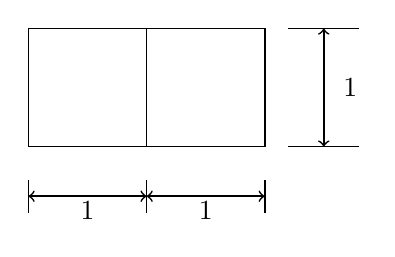
\begin{tikzpicture}[scale=1.5, semithick]
  % 正视图：宽 2、高 1，中间一条竖线
  \draw (0,0) -- (2,0) -- (2,1) -- (0,1) -- cycle;
  \draw (1,0) -- (1,1);

  % 下方两段宽度标注
  \draw[<->] (0,-0.42) -- (1,-0.42);
  \draw (0,-0.56) -- (0,-0.28);
  \draw (1,-0.56) -- (1,-0.28);
  \node[below] at (0.5,-0.38) {$1$};
  \draw[<->] (1,-0.42) -- (2,-0.42);
  \draw (2,-0.56) -- (2,-0.28);
  \node[below] at (1.5,-0.38) {$1$};

  % 右侧高度标注
  \draw[<->] (2.5,0) -- (2.5,1);
  \draw (2.2,0) -- (2.8,0);
  \draw (2.2,1) -- (2.8,1);
  \node[right] at (2.58,0.5) {$1$};
\end{tikzpicture}
